
\chapter{Storm: A quick introduction}

It will be hard to review the code of the platform if the reader does not have
any clue about Storm, and how Storm applications work. This is why I have
written this appendix. It is probably not the most complete tutorial on Storm,
but I believe that it gives the reader a quick and easy to follow introduction
to Storm.

For this reason, I have added a directory called ``storm-example'' in the root
of the project. In this directory there is a file called BasicTopology.scala.
This file contains the easiest example that I could think of about Storm:
counting words. In this example we have one spout and two bolts. The spout
sends random sentences from a pool of sentences. The output of this spout is
sent to the first bolt (called {\bf SplitSentence}). This bolt will split the
sentence into words and send the words to the last bolt. The last bolt (called
{\bf WordCount}) keeps track of the words that it has tracked so far. When to
WordCount bolt receives a word, this word is printed to the standard output,
followed by a number (representing how many times this word has been counted).
Therefore, this is the {\bf topology} of this example:

\begin{figure}[H]
  \centering
  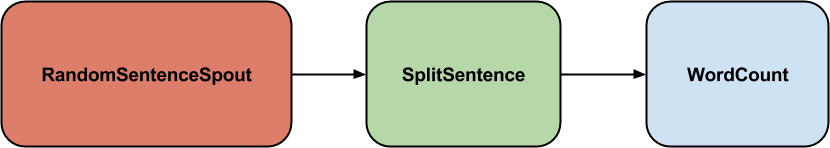
\includegraphics[scale=0.5]{images/example.png}
  \caption{The topology of the Storm example}\label{fig:example}
\end{figure}

Let's dig into the code. First of all we will take a look at the
RandomSentenceSpout. The code for this spout is shown by the figure
\ref{fig:randomsentencespout}.

\begin{figure}
  \centering
  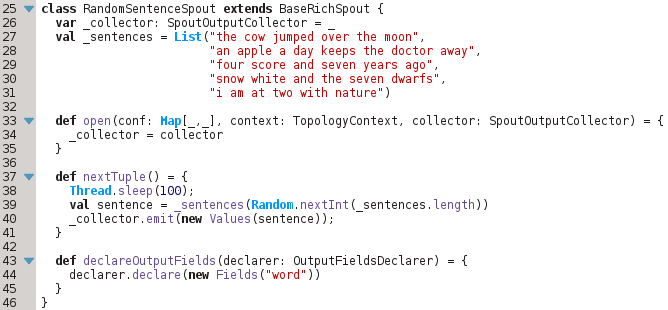
\includegraphics[scale=0.8]{images/randomsentencespout.png}
  \caption{The code of the RandomSentenceSpout}\label{fig:randomsentencespout}
\end{figure}

A Spout in Storm has to inherit from the BaseRichSpout. After doing this, it
has to implement three methods:

\begin{enumerate}
  \itemsep0em
  \item {\bf open}: this method will be called each time that the bolt is
opened. We can initialize our bolt here. In the most simple case, we just need
to initialize our instance of the SpoutOutputCollector class.
  \item {\bf nextTuple}: this method will be called everytime that Storm needs
a new value from this spout.
  \item {\bf declareOutputFields}. This method is the glue between this spout
and the next bolt. It declares the number and the names of the fields that will
be sent as the output. Note that the number and type of output values have to
match the ones given by the ``\_collector.emit'' call inside the nextTuple
function.
\end{enumerate}

Now let's see the bolts. The first bolt is the one the splits the given
sentences into words. The code for this bolt is shown in figure
\ref{fig:splitsentence}.

\begin{figure}
  \centering
  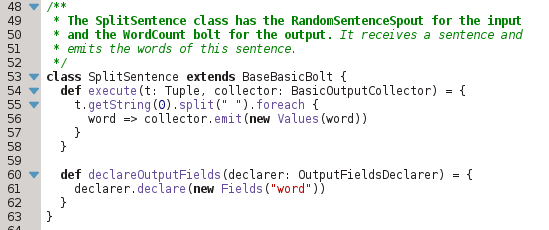
\includegraphics[scale=0.8]{images/splitsentence.png}
  \caption{The code of the SplitSentence bolt}\label{fig:splitsentence}
\end{figure}

As you can see from the SplitSentence's code, bolts are even simpler than
spouts. In this case, this bolt is a subclass of the class {\bf BaseBasicBolt}.
A bolt only has to implement two functions:

\begin{enumerate}
  \itemsep0em
  \item {\bf execute}: this function will be called when this bolt has received
some input. In this case the input is a sentence. The execute function will
emit each word to the next bolt.
  \item {\bf declareOutputFields}: it is the same as we have seen from the
RandomSentenceSpout.
\end{enumerate}

The last bolt receives each word and has to count it. You can see the code of
this bolt in the figure \ref{fig:wordcount}.

\begin{figure}
  \centering
  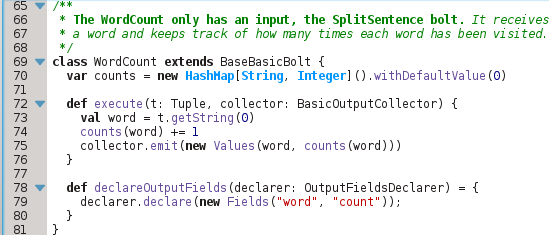
\includegraphics[scale=0.8]{images/wordcount.png}
  \caption{The code of the WordCount bolt}\label{fig:wordcount}
\end{figure}

As you can see, there is nothing special about the WordCount bolt. Also note
that the declareOutputFields method has to be implemented even if there are no
more bolts listening to the output of the WordCount bolt. This output will be
logged into the standard output.

We have now the three classes ready. Now it is time to use them in the main
function. The main function is shown in figure \ref{fig:example_main}.

\begin{figure}
  \centering
  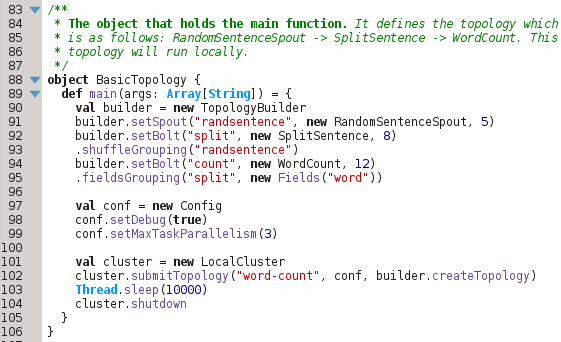
\includegraphics[scale=0.8]{images/main.png}
  \caption{The code of the main function}\label{fig:example_main}
\end{figure}

As you can see, the first thing that we do in the main function is to create a
new {\bf TopologyBuilder}. With this builder we can form a topology. As I have
already said, the topology that we are going to setup is the same as figure
\ref{fig:example}. Nonetheless, note that with these same spout and bolts we
could perfectly have different topologies. For example: we could create a
topology consisting of one spout, 2 SplitSentence bolts and 1 WordCount bolt.
This would work just fine because the classes for spouts and bolts are totaly
unaware of the topology. This flexibility is one of the most valuable
advantages of Storm over other alternatives.

After building the topology, we setup the number of task parallelism. After
this, we will submit the newly created topology. We will run this topology for
10 seconds, and then we are shutting it down.

This is all the code that we need for this example. It is simple,
straightforward and fast. Now it is time to run this application to see how it
actually performs. To do this we will be using the SBT toolchain. As you can
see, there is already a configuration file for SBT for this project. This file
is named ``build.sbt''. Take a look at some of the options.

In order to run this application we will simply perform the following commands:

\begin{center}
  \$ sbt \\
  $>$ run
\end{center}

If it is the first time that you run this application, it will automatically
download and install all the dependencies for you. The ``run'' command compiles
the project and then it runs the executable main function.

If everything went according to plan, you should see an output like the one
shown in figure \ref{fig:example_output}. I have highlighted in red some of the
results.

\begin{figure}
  \centering
  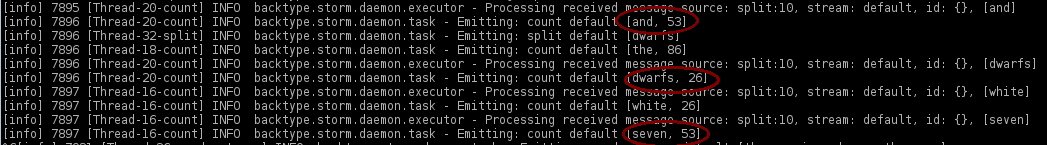
\includegraphics[scale=0.6]{images/example_output.png}
  \caption{The output from the Storm example}\label{fig:example_output}
\end{figure}
